% ---
% Capitulo de METODOLOGIA
% ---


\chapter{Metodologia}\label{cap:metodologia}
Nesta seção apresenta-se os materiais e métodos utilizados no desenvolvimento do trabalho proposto.
\section{Materiais e Métodos}

O presente estudo classifica-se como uma pesquisa experimental, a pesquisa experimental segundo \cite{wazlawick2017metodologia} condiciona o pesquisador a lidar com diversas variáveis experimentais e variáveis observacionais visando levar possivelmente, correlações e dependências entre as elas, utilizando de técnicas de amostragem e testes de hipóteses. O mesmo diz que trabalhos desenvolvidos em cima de abordagens padronizadas e aceitas internacionalmente, apresentando dados empíricos é relevantes, se encaixam no nível mais maduro de pesquisa, onde o autor deverá apresentar os resultados usando métricas aceitas pela comunidade, através de observações e medições, implicando que o pesquisador provocará alterações sistemáticas no ambiente do experimento para se observar os resultados após cada intervenção produzida.

\subsection{Materiais}

Para a implementação do método de intervalo de confiança, além da realização dos testes com dados em tempo real, utilizou-se dos seguintes materiais citados a seguir na tabela.

\begin{longtable}{|p{4cm}|p{3.5cm}|}
    \hiderowcolors
    \caption{Equipamentos utilizados}
    \label{tab:makespan}\\
    \showrowcolors
    \hline
    \rowcolor[HTML]{C0C0C0} 
    \multicolumn{1}{c|}{\cellcolor[HTML]{C0C0C0}\textbf{EQUIPAMENTO}} & \multicolumn{1}{c|}{\cellcolor[HTML]{C0C0C0}\textbf{UNIDADE}} \\ \hline

    \endfirsthead
    \rowcolor[HTML]{C0C0C0} 
    \multicolumn{1}{c|}{\cellcolor[HTML]{C0C0C0}\textbf{EQUIPAMENTO}} & \multicolumn{1}{c|}{\cellcolor[HTML]{C0C0C0}\textbf{UNIDADE}} \\ \hline

    \endhead
		\hline
		\textcolor[rgb]{0.125,0.129,0.141}{ESP32-DevKitC ESP-WROOM-32U} & 1                \\
		\hline
		\textcolor[rgb]{0.059,0.067,0.067}{Cabo USB-Micro USB}          & 1                \\
		\hline
		Protoboard 400 pontos                                           & 1                \\
		\hline
		Sensor de temperatura termistor de 100k                         & 1                \\
		\hline
    
    \end{longtable}

\section{Tabela de referencias}
Aqui serão apresentados os 5 artigos recentes relacionados a esse trabalho, tendo suas vantagens e desvantagens levantadas com relação aos seus métodos propostos e uma breve descrição do trabalho.

\begin{longtable}{|p{2cm}|p{4cm}|p{3.5cm}|p{3.5cm}|}
    \hiderowcolors
    \caption{Referências bibliográficas}
    \label{tab:makespan}\\
    \showrowcolors
    \hline
    \rowcolor[HTML]{C0C0C0} 
    \multicolumn{1}{c|}{\cellcolor[HTML]{C0C0C0}\textbf{Trabalhos analisados}} & \multicolumn{1}{c|}{\cellcolor[HTML]{C0C0C0}\textbf{Objetivo}} & \multicolumn{1}{c|}{\cellcolor[HTML]{C0C0C0}\textbf{Vantagens}} & \multicolumn{1}{c|}{\cellcolor[HTML]{C0C0C0}\textbf{Desvantagens}} \\ \hline

    \endfirsthead
    \rowcolor[HTML]{C0C0C0} 
    \multicolumn{1}{c|}{\cellcolor[HTML]{C0C0C0}\textbf{Trabalhos analisados}} & \multicolumn{1}{c|}{\cellcolor[HTML]{C0C0C0}\textbf{Objetivo}} & \multicolumn{1}{c|}{\cellcolor[HTML]{C0C0C0}\textbf{Vantagens}} & \multicolumn{1}{c|}{\cellcolor[HTML]{C0C0C0}\textbf{Desvantagens}} \\ \hline

    \endhead
    \hline
    \cite{Arab_LSTM_ResNet} &   O trabalho propõe utilizar uma técnica de aprendizado profundo para classificar e eliminar ruídos de sistemas de comunicação via micro-ondas, aproveitando-se da aptidão do algoritmo em se adestrar se com os dados coletados em tempo real.	& Algoritmo pode ser treinado em tempo real e acompanhar diferentes tipos de ruídos. & Necessita de uma grande quantidade de dados já coletados para treinamento, exigência de grande capacidade de recurso de computação. \\ \hline
   
    \cite{Kamata_mems} &   O seguinte estudo propõe uma filtragem para processamento de sinal de um componente eletrônico giroscópio embarcado e avaliando seu desempenho. &   A técnica pode ser utilizada também para acelerômetros, e viabiliza o uso de componentes de custo baixo e alta precisão. & Limitasse a um ambiente de sensores específicos. \\ \hline
    
    \cite{Ning_magnetometer} &   Aqui os autores implementa uma combinação de filtros para eliminar dados ruidosos em tempo real e compensar a interferência dos erros de um sensor magnético, utilizando de diversos métodos como Auto-Regressão e Média móvel, para modelar a medição de ruído, a fim de excluir dados errados do resultado final. &   O método utilizado é adaptativo e abrangente, podendo resolver ruídos dinamicamente. & Os testes não foram realizados durante o processo de coleta de dados. \\ \hline
    
    \cite{Kaan_emg} &   Aqui é proposto um novo método de processamento de dados de sensores de eletromiografia sensível, utilizando um algoritmo adaptativo em tempo real para eliminar os ruídos provindos de fontes elétricas de corrente alternada, sem perturbar os dados reais do sensor, ao qual conseguiu superar cinco alternativas existentes de última geração para tratamento de sinal de eletromiografia, mantendo a qualidade do sinal.  &  Seu comportamento adaptativo exibe uma vantagem em manter os dados coletados o mais próximo possível dos dados reais, sem diminuir a potência do sinal. & Por estar no estado da arte, ainda não apresenta outros estudos comprovando sua utilização em tempo real. \\ \hline
    
    \cite{Zhou_ambient} &   Os autores apresentam um método que combina processamento de sinal e cancelamento de ruído adaptativo para filtrar e eliminar interferências do ambiente. Duplicando o sinal recebido em dois canais diferentes, sobrepondo um sobre o outro e eliminando as interferências em ambos de forma a evitar perdas dos espectros. &   Identifica sinais de interferência utilizando uma quantidade inferior de dados. & Quanto maior a sobreposição, maior a carga computacional necessária para processar os canais diferentes. \\ \hline
    
\end{longtable}


% Reescrever
% O presente estudo classifica-se como uma pesquisa experimental, em que os experimentos foram realizados
% para avaliar o desempenho do Sistema de tempo real Zephyr\cite{Zephyr}
% versão 1.14 no microcontrolador ESP32-WROOM-32D de 32 Bits, dois cores e 240MHz, em fatores como analise
% de interrupções, sincronização e compartilhamento de recursos e passagem de mensagem
% entre outras tarefas mais voltadas para o contexto da missão de um cubesat como alocação em memoria flash.

% Foi escolhido o sistema \cite{Zephyr} como alternativa, pois o
% mesmo tende a ser um dos mais promissores a ser competitivos perante o FreeRTOS, o benchmark usado é
% baseado nos critérios propostos e chamados de benchmarks refinados em \cite{Garcia}, mas também se baseia
% na metodologia mais moderna realizada por \cite{Raymundo} no qual apresenta um trabalho muito similar e
% completo, mas focado em tecnologias para internet das coisas. Com o objetivo de avaliar se o \cite{Zephyr}
% tem qualidade perante a ao FreeRTOS, outro sistema operacional de tempo real mais popular na industria de
% cubesats de codigo aberto.

% A pesquisa experimental segundo \cite{wazlawick2017metodologia} condiciona o pesquisador a lidar com
% diversas variáveis experimentais e variáveis observacionais, visando levar possivelmente, correlações
% e dependencias entre as elas, utilizando de técnicas de amostragem e testes de hipóteses.
% O mesmo diz que trabalhos desenvolvidos em cima de abordagens padronizadas e
% aceitas internacionalmente, apresentando dados empíricos é relevantes, se encaixam no nível mais maduro
% de pesquisa, onde o autor deverá apresentar os resultados usando métricas aceitas pela
% comunidade, através de observações e medições, implicando que o pesquisador provocará alterações sistemáticas
% no ambiente do experimento para se observar os resultados após cada intervenção produzida.

% % Questão
% % O zephyr rtos tem qualidade perante a outros rtos do 
% % mercado na plataforma ESP32?



\subsection{Análise exploratória dos dados}
É utilizado no presente trabalho um conjunto de dados coletados através do sensor de temperatura termistor de 100k acomodado no pino 21 do microcontrolador esp32. 

O conjunto de dados coletados contém 1592 linhas sem valores ausentes e 544 valores únicos com os valores \ang{32.14}c e \ang{33.47}c sendo os que mais se repetem com 35 aparições, todos os valores flutuando entre \ang{1.05}c e \ang{97.35}c graus, tendo média de \ang{37.19}c, desvio padrão de 13.33, primeiro quartil de 31.80, segundo quartil 33.00 e terceiro quartil em 35.33.
Os valores foram coletados no intervalo de aproximadamente 2 minutos, com todos os valores sendo processados em python com as bibliotecas pandas, numpy, matplotlib e scipy.


Na Figura~\ref{fig: hist} abaixo visualiza-se uma concentração maior de valores entre \ang{20}c e \ang{40}c graus com os valores seguintes podendo estar entre ruídos e picos de temperatura capturados pelo sensor. 

\begin{figure}[H]
	\centering
	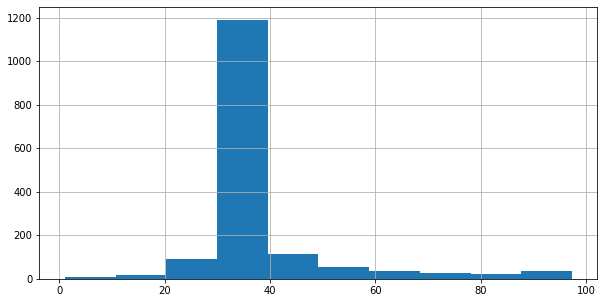
\includegraphics[width=15cm]{imagens/sensores/hist.png}
	\caption{histograma do conjunto de dados}
	Fonte: Autor com base na biblioteca pandas.
	\label{fig: hist}
\end{figure}

Tendo em vista que a média de temperatura do local de coleta da amostra estava entre \ang{33}c graus, podemos visualizar uma grande quantidade de valores aproximados na Figura~\ref{fig: hist2}. 

\begin{figure}[H]
	\centering
	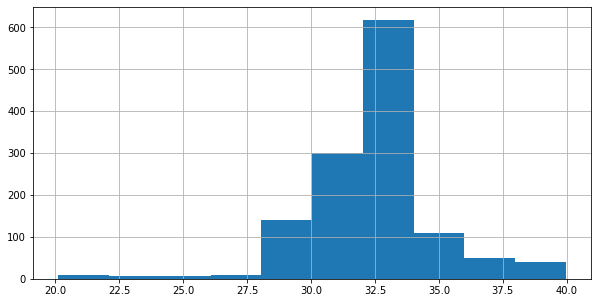
\includegraphics[width=15cm]{imagens/sensores/hist2.png}
	\caption{histograma do conjunto de dados entre 20 e 40 graus}
	Fonte: Autor com base na biblioteca pandas.
	\label{fig: hist2}
\end{figure}

\begin{figure}[H]
	\centering
	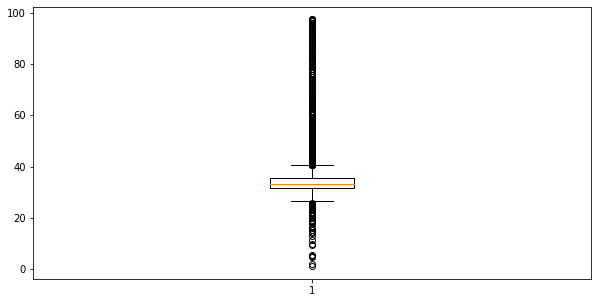
\includegraphics[width=15cm]{imagens/sensores/boxplot.png}
	\caption{Boxplot do conjunto de dados}
	Fonte: Autor com base na biblioteca matplotlib.
	\label{fig: boxplot}
\end{figure}

Verifica-se na Figuras~\ref{fig: boxplot} a grande presença de valores discrepantes acima de \ang{40}c e abaixo de \ang{20}c.

Abaixo na Figura~\ref{fig: bruto} podemos visualizar todo o conjunto de dados, nota-se a presença de grandes picos de temperatura que foram induzidos na amostra propositalmente a fim de diferenciar o ruído do sensor de um pico de temperatura real, esses picos foram introduzidos através do aquecimento do sensor de temperatura duas vezes durante a coleta de dados.


\begin{figure}[H]
	\centering
	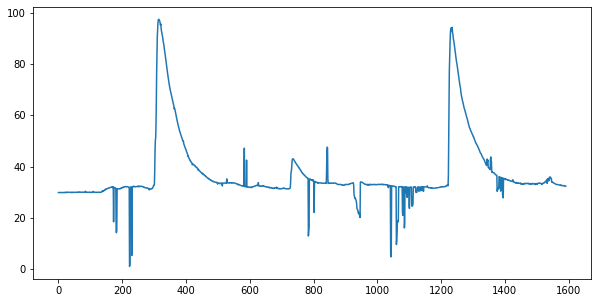
\includegraphics[width=15cm]{imagens/sensores/bruto.png}
	\caption{Plotagem gráfica do conjunto de dados completo}
	Fonte: Autor.
	\label{fig: bruto}
\end{figure}

As linhas verticais discrepantes indicam possíveis ruídos, onde a temperatura alcançou valores muito diferentes em períodos extremamente curtos. Esses ruídos podem ter sido gerados por baixa qualidade do termistor ou pela exposição ao ambiente dos fios de conexão entre o termistor e o microcontrolador.


\begin{figure}[H]
	\centering
	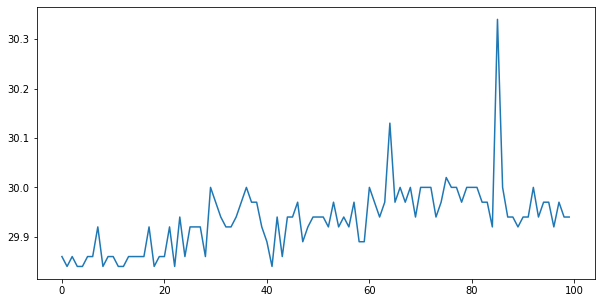
\includegraphics[width=15cm]{imagens/sensores/bruto_100_primeiras}
	\caption{Plotagem gráfica das 100 primeiras linhas do conjunto}
	Fonte: Autor.
	\label{fig: bruto_100p}
\end{figure}

Na Figura~\ref{fig: bruto_100p} percebe-se que a leitura do sensor sempre apresenta alguma variação, por mais pequena que seja, essa pequena diferença na coleta de dados pode não significar um problema, podendo ser tratada através de um simples cálculo de média. A criticidade dessa variação deve ser avaliada em cada projeto, com os dados ruidosos muito fora da média e esporádicos, interferindo significativamente no resultado final.

\begin{figure}[H]
	\centering
	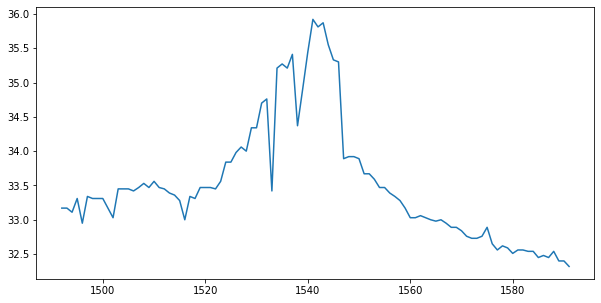
\includegraphics[width=15cm]{imagens/sensores/bruto_100_ultimas.png}
	\caption{Plotagem gráfica das 100 ultimas linhas do conjunto}
	Fonte: Autor.
	\label{fig: bruto_100u}
\end{figure}

Por fim na Figura~\ref{fig: bruto_100u} podemos analisar os últimos 100 dados, nos quais nota-se a presença de um pico de temperatura que começa a subir em \ang{33.05}c com sua máxima perto dos \ang{36.0}c, essa característica pode ser importante por mais que esteja em um curto período de tempo, e pode ser distinguida de um ruído pela sua característica de subida e descida prolongada. 

O algoritmo utilizado neste trabalho é bem simples, um vetor é responsável por guardar os últimos valores coletados para realizar o cálculo de intervalo de confiança, uma variável define o tamanho da amostra. Com o vetor completamente preenchido e o cálculo realizado, o algoritmo verifica se o dado coletado se encontra dentro do espaço entre os dois intervalos, caso seja contemplado o valor é adicionado a variável de resultado ao qual finaliza o laço de repetição sendo assim retornado ao fim do algoritmo, caso não seja contemplado o algoritmo segue em ritmo contínuo até encontrar um resultado verdadeiro.

\begin{algorithm}[H]
    \Entrada{Tamanho do vetor de amostras ($TV$), Vetor de amostras ($VA$)}
    \Saida{Valor considerado verdadeiro ($resultado$), Vetor de amostras ($VA$)}
    \Inicio{
		\While{$resultado == SemValor$}{
			$V \leftarrow coletaDadoDoSensor()$; \tcc*[f]{Coleta dado do sensor} \\

			% \tcc*[f]{Verifica se o vetor já foi completamente preenchido} \\
			\Se{$tamanho(VA) \geq TV$}{ 

				% \tcc*[f]{Retira intervalo de confiança} \\
				$primeiroIntervalo$, $segundoIntervalo \leftarrow intervaloDeConfianca($VA$)$; 

				% \tcc*[f]{Verifica se o valor está dentro do intervalo de confiança} \\
				\Se{$V \geq primeiroIntervalo$ \&\& $V \leq segundoIntervalo$}{
					$resultado \leftarrow V$; %\tcc*[f]{Adiciona o valor ao retorno} \\
				}
				
				$VA \rightarrow primeiroElemento$; \tcc*[f]{Remove elemento mais velho} \\
			}

			$VA \leftarrow V$; \tcc*[f]{Adiciona valor para dentro do vetor de amostra} \\
		}


		\tcc*[f]{Retorna valor verdadeiro e vetor com as últimas amostras} \\
		\Retorna $resultado$, $VA$; 
    }
    \caption{Algoritmo para coleta de valor considerado verdadeiro dentro do intervalo de confiança}
    \label{algoritmo:makespan}
\end{algorithm}


% A Figura~\ref{fig: ESP-IDF Software} mostra as principais fases para construir uma aplicação em 
% ESP32, abaixo em ESP-IDF encontra-se as bibliotecas e códigos fontes para operar a segunda camada, 
% chamada de Toolchain, contem todas as ferramentas para compilação de código que através de ferramentas 
% de compilação de projeto externas como CMake e Ninja controem a aplicação final.

% \begin{figure}[H]
% 	\centering
% 	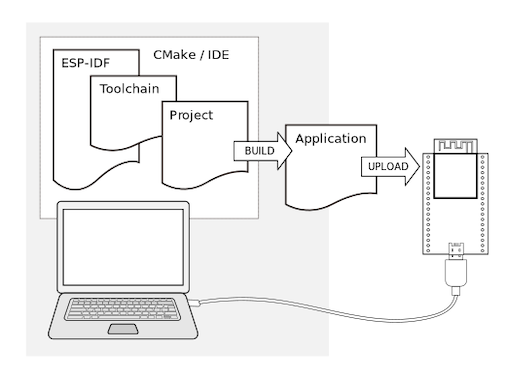
\includegraphics[width=15cm]{imagens/what-you-need.png}
% 	\caption{Diagrama do processo de construção de uma aplicação para ESP32.}
% 	Fonte: Retirado de ESP-IDF Programming Guide em https://docs.espressif.com/projects/esp-idf/en/latest/esp32/get-started/index.html
% 	\label{fig: ESP-IDF Software}
% \end{figure}

% Todo esse ambiente foi motado na IDE Visual Studio Code, utilizando o plugin PlataformIO para 
% desenvolvimento em dispositivos embarcados. A instalação do Zephyr requer diversos passos, para 
% facilitar esse processo foi desenvolvido um script de instalação na linguagem Shell Script, o mesmo 
% foi disponibilizado no site github em 
% \footnote{https://gist.github.com/talesmm14/148b9e02966b038f9334dcbbc4c5451a} para consulta.


% % 1 Descrição do objetivo do estudo
% % 2 Delineamento da pesquisa
% %\subsection{Implementação dos métodos}

% %\subsection{Métricas}
% \section{Critérios de avaliação}
% Segundo \cite{Garcia} existe uma necessidade de avaliação de desempenho de
% sistemas de computador em tempo real, pois os mesmos devem operar em
% períodos de tempos determinísticos em aplicações críticas. Diante disto
% realizaremos os seguintes testes de performance.

% \subsection{Velocidade de troca entre tarefas}
% Uma tarefa de prioridade mais alta permanece dormente, em quanto a segunda tarefa
% com prioridade inferior desperta a primeira tarefa, o tempo de mudança entre as
% tarefas e medido.

%Algoritmo Soma Ponderada


% \subsection{Tempo de passagem de mensagens entre tarefas}
% Uma tarefa será responsável por enviar as mensagens para uma fila vazia, outra
% tarefa ira receber a mensagem, o tempo de envio e recebimento das mensagens e
% medido.

% \begin{figure}[H]
% 	\centering
% 	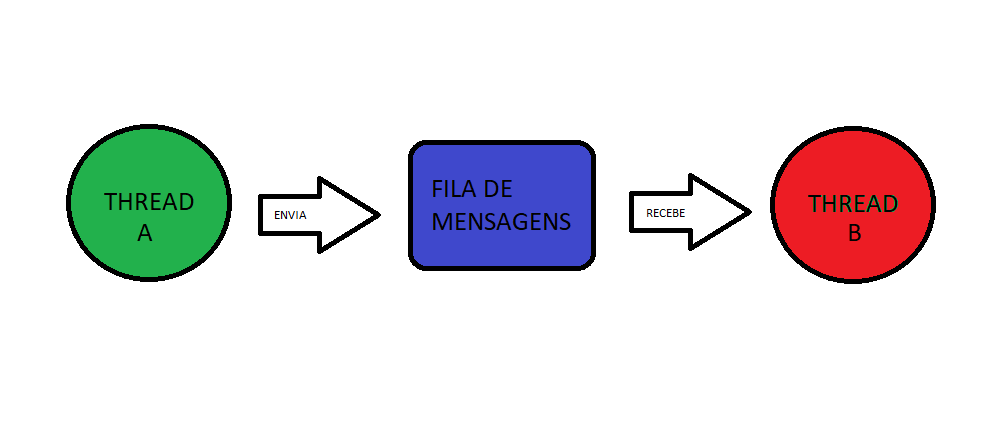
\includegraphics[width=15cm]{imagens/fila_mensagens.png}
% 	\caption{A tarefa A envia uma mensagem, a tarefa B recebe.}
% 	Fonte: Autoria Própria.
% 	\label{fig: fila_mensagens}
% \end{figure}

% Uma tarefa de prioridade maior solicita uma mensagem de uma fila vazia, uma tarefa
% de prioridade menor enviar a mensagem, o tempo de solicitação e envio de mensagem e
% medido.

% \subsection{Tempo de bloqueio e liberação de desbloqueio de Semáforo e Mutex}
% Uma tarefa solicita e libera em seguinte um semáforo, o tempo de bloqueio e
% liberação do semáforo são medidos, o mesmo teste e realizado com um Mutex.

% \begin{figure}[H]
% 	\centering
% 	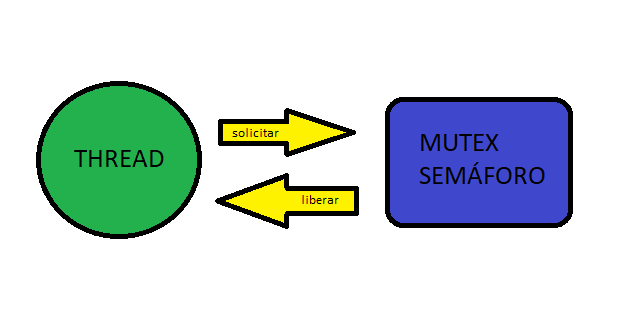
\includegraphics[width=15cm]{imagens/solicitar_bloquear.png}
% 	\caption{A tarefa solicita e libera uma variável de controle.}
% 	Fonte: Autoria Própria.
% 	\label{fig: tempo_semaforo_mutex}
% \end{figure}

% Uma tarefa de prioridade mais alta solicita o semáforo já bloqueado por uma
% tarefa de prioridade inferior, o tempo em que ocorre a mudança entre as tarefas
% é medido, o mesmo teste e realizado com um Mutex.

% \subsection{Tempo de resposta a eventos externos atraves de interrupção}
% Nesse teste será medido o tempo de latência de despacho de uma rotina de serviço de interrupção (ISR) 
% e o tempo de despacho de uma tarefa desbloqueada por uma interrupção gerada por um estimulo
% externo.

% \subsection{Velocidade de alocação de memoria}
% Uma tarefa realiza a alocação de espaço na memoria de tamanho fixo de acordo com
% as especificações do microcontrolador ESP32, em seguida liberando a memoria,
% o tempo de alocação e desbloqueio de memoria são medidos.

% \subsection{Velocidade de leitura e gravação em memoria flash (Cartão SD)}
% Uma tarefa adquire uma região de espaço na memoria flash disponivel, a mesma gravará
% uma quantidade de dados especifica e liberar esta região da memoria, o tempo de adquirir
% o espaço, gravar os dados e liberar a memoria serão medidas.


% \subsection{Configuração de hardware}
% %Aqui serão apresentados os equipamentos utilizados para a elaboração desta pesquisa.

% \begin{table}[]
% 	\centering
% 	\begin{tabular}{|l|l|}
% 		\hline
% 		\textbf{EQUIPAMENTO}                                            & \textbf{UNIDADE} \\
% 		\hline
% 		\textcolor[rgb]{0.125,0.129,0.141}{ESP32-DevKitC ESP-WROOM-32U} & 1                \\
% 		\hline
% 		\textcolor[rgb]{0.059,0.067,0.067}{Cabo USB-Micro USB}          & 1                \\
% 		\hline
% 		Protoboard 400 pontos                                           & 1                \\
% 		\hline
% 	\end{tabular}
% 	\caption{Equipamentos utilizados}
% \end{table}

% O Hardware escolhido para realizar este estudo foi o ESP32 por possuir varias caracteristicas 
% interessantes para uma missão espacial, como temperatura de trabalho de -40° á +85° C, por 
% ter dois nucleos e 32-bit, suas configurações de memoria são muito atraentes com 448 KBytes de 
% memoria ROM, 520 KBytes de RAM e 4MB de memoria Flash, possui também diversas portas 
% GPIO com funções de PWM, I2C, SPI, etc e por ultimo um baixo consumo de corrente de 80mA típica 
% e 500mA máxima. Este equipamento foi escolhido por ser de custo baixo, muito utilizado em projetos 
% de pequenos satelites e de documentação de facil acesso além de ser compatível com a IDE do Arduino 
% permitindo uma simples adoção por toda a comunidade.



% \subsection{Medida de tempo}

% Para a realização deste benchmark destaca-se a preocupação com a metodologia usada para medir o tempo 
% de cada experimento, assim de acordo com a fabricante \cite{} {Expressif} os temporizadores de hardware apresentam 
% vantagens em relação aos mesmos implementados em software, um exemplo disto seria que o \cite{FreeRTOS} 
% forneçe temporizadores com algumas limitações como a resolução máxima de é igual ao período de ticks 
% do próprio sistema operacional, outra limitação está no retorno da chamada do temporizador que são entregues 
% por uma tarefa de baixa prioridade, no qual pode conflitar com outras tarefas do sistema. 



